\documentclass[../thesis/thesis.tex]{subfiles}
\begin{document}

\chapter{Design}
\label{chap:design}

In this chapter, we explain the methodology used to fill the research gap identified in Chapter~\ref{chap:litreview}, thereby producing a system that identifies high-potential startup companies that are likely to receive additional funding or a exit in a given forecast window. Figure~\ref{fig:design:system_architecture} depicts the overall system architecture. The first two steps are our designed system and will be described in this chapter. The following two steps are part of our system evaluation process and will be described in the next chapter, Chapter~\ref{chap:evaluation}.

\begin{figure}[!htb]
    \centering
    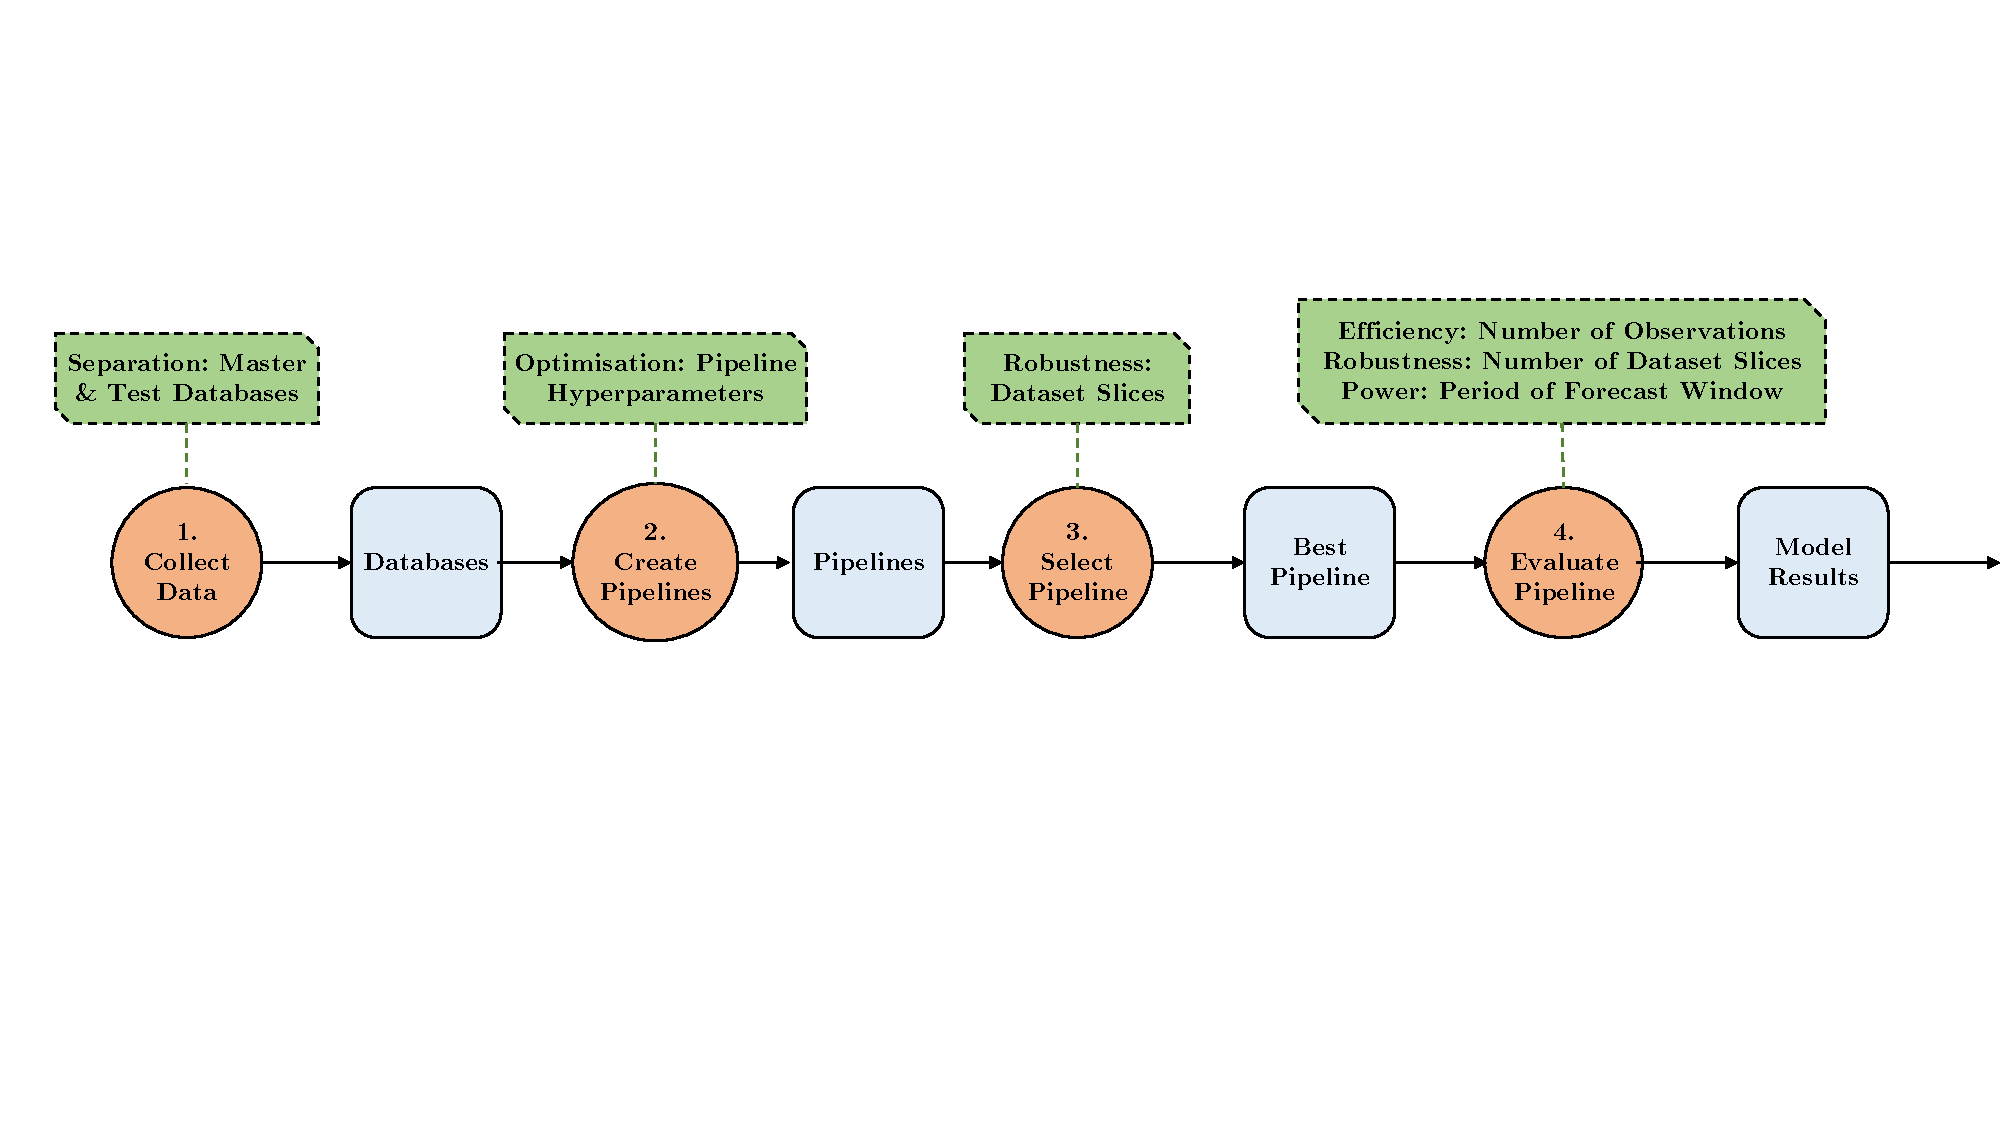
\includegraphics[width=\textwidth]{../figures/design/system_architecture}
    \caption[System architecture flowchart]{An overview of the system architecture proposed by this project, structured in four stages: data collection, pipeline creation, pipeline selection, and model evaluation. Green callouts: iterative processes / search spaces. Orange circles: linear systems. Blue squares: data structures / data stores.}
    \label{fig:design:system_architecture}
\end{figure}

\begin{enumerate}

\item Dataset Preparation. Our primary data source was the CrunchBase online database, which we supplemented with patent filing data from PatentsView. We collected two database dumps from CrunchBase in September 2016 and April 2017, for training and testing respectively. The database dumps were in the format of CSV files which we imported into a relational database (SQLite) and performed aggregation queries to create features suitable for classification. We then performed screening based on each company's developmental stage and age to ensure only relevant companies were included in the dataset. Finally, we explored the dataset and identified issues of sparsity, long-tailed distributions, imbalanced feature ranges, and non-orthogonality.

\item Pipeline Creation. We developed a processing pipeline framework that seeks to address the dataset issues identified during data collection. Our pipeline is based on the popular Python machine learning library Scikit-learn \cite{pedregosa2011}. Pre-processing steps include imputation, transformation, scaling and feature extraction. Each pre-processing step has hyperparameters that can be tuned (e.g. imputation strategy, number of components to extract) that affect the pipeline's classification performance. We also tested a number of common classification algorithms and their hyperparameters, selected from our literature review in Chapter~\ref{chap:litreview}. We performed a search across the pipeline's hyperparameters to generate candidate pipelines. The hyperparameters that we found to have the most significant effect on the final performance of the pipelines were related to the classification algorithms.

\end{enumerate}

\section{Dataset Preparation}

In the previous chapter, we reviewed the literature concerning data sources for entrepreneurship and \gls{vc} investment. We concluded the most promising primary data sources for this project are CrunchBase and AngelList, for their size, comprehensiveness and ease of access. We suggested PatentsView (the online database of the US Patent Office) could be a useful secondary data source for structural capital features. In the following sections, we first discuss how we collected data from CrunchBase and PatentsView, converted the relational databases into a format suitable for machine learning, performed preliminary screening to ensure we only included relevant companies. This process is depicted in Figure~\ref{fig:design:data_collection}. Following our description of this process we describe the results of exploratory analysis on our dataset and identify dataset issues which will be addressed in later steps.

\begin{figure}[!htb]
    \centering
    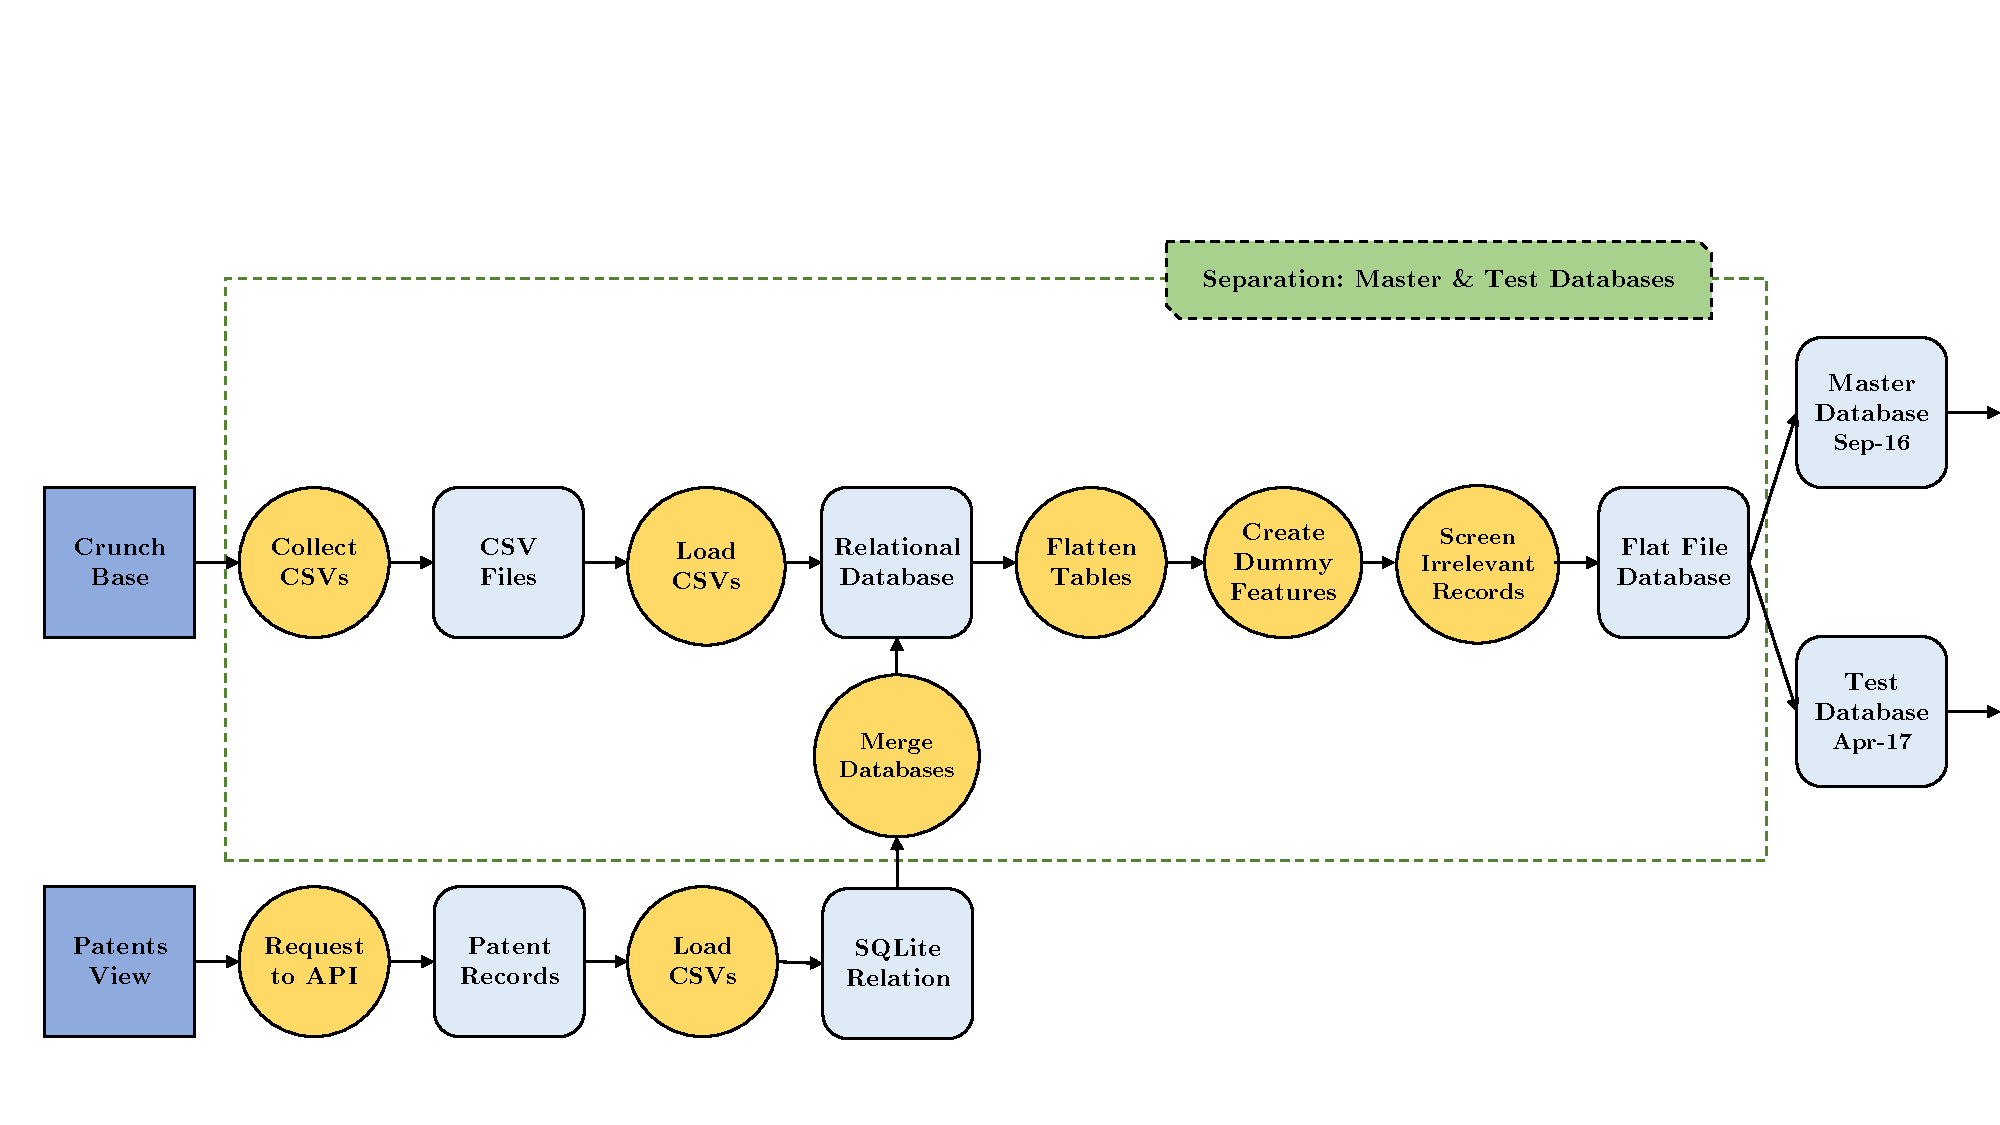
\includegraphics[width=\textwidth]{../figures/design/data_collection}
    \caption[Data collection flowchart]{Data collection overview.}
    \label{fig:design:data_collection}
\end{figure}


\subsection{Data Collection}

\subsubsection{CrunchBase}

CrunchBase is an online, crowd-sourced repository of startup companies, individuals and investors with a focus on US high-tech sectors. CrunchBase is freely accessible for browsing but requires licenses to filter the dataset, use the API, and download Microsoft Excel and CSV-formatted dumps. For the purposes of this project, we were granted an Academic License. CrunchBase provides database access in a few formats that offer trade-offs in terms of accessibility and comprehensiveness. We intended to use CrunchBase's API because it provides the most comprehensive access to their database. We developed a collector that downloaded a daily list of updated API endpoints from CrunchBase and queried nodes it needed to update. CrunchBase's API provides JSON-formatted responses which the program recursively parsed and stored into a relational database. However, due to the time constraints of this research project, we abandoned this data collection method. CrunchBase also provides CSV-formatted dumps of their key endpoints (e.g. organizations, people, funding rounds). We downloaded two CSV-formatted dumps from Crunchbase on 09 September 2016 and 04 April 2017 which we loaded into relational databases (see Appendix~\ref{appendix:database_schema} for the full database schema).

\subsubsection{PatentsView}

In 2015, the \gls{uspto} launched PatentsView, a free public API to allow programmatic access to their database. PatentsView holds over 12 million patent filings from 1976 onwards \cite{schultz2016}. The database provides comprehensive information on patents, their inventors, their organisations, and locations. We collected the patent filing records of each company in the primary database, focusing on information relating to dates, citations, and patent types. We matched the data sources on standardised company names (removing common suffixes, punctuation etc.) and using normalised Levenshtein distances. Although approximate matching introduces error, the volume of companies in the database is too high to be matched manually and there are no other identifying records. We stored the PatentsView data in a relation which we merged into our master and test databases.

\subsection{Dataset Manipulation}

To prepare the dataset for machine learning, we first flattened the relational database into a single file using SQL aggregation queries. We aggregated each relevant relation in turn, grouping by Company ID and then combined each aggregated table using left outer joins. Following this process, we used Python to convert tuples (e.g. Round Type and Round Date) and lists (e.g. Round Types) into dummy variables.

We performed preliminary screening on the primary dataset (N = 425,934) to ensure it only included relevant companies. We were interested in removing traditional, non-startup businesses from the dataset (e.g. consulting firms, companies that will not take \gls{vc} funding etc.). To do this, we explored two factors for each company: developmental stage and age. By developmental stage, we primarily refer to external funding milestones. These stages are associated with shifts in a startup company's functions and objectives and we also expect them to correlate with company age. Our dataset as grouped by startup developmental stage is depicted in Figure~\ref{fig:design:lifecycle}.

\begin{figure}[!htb]
    \centering
    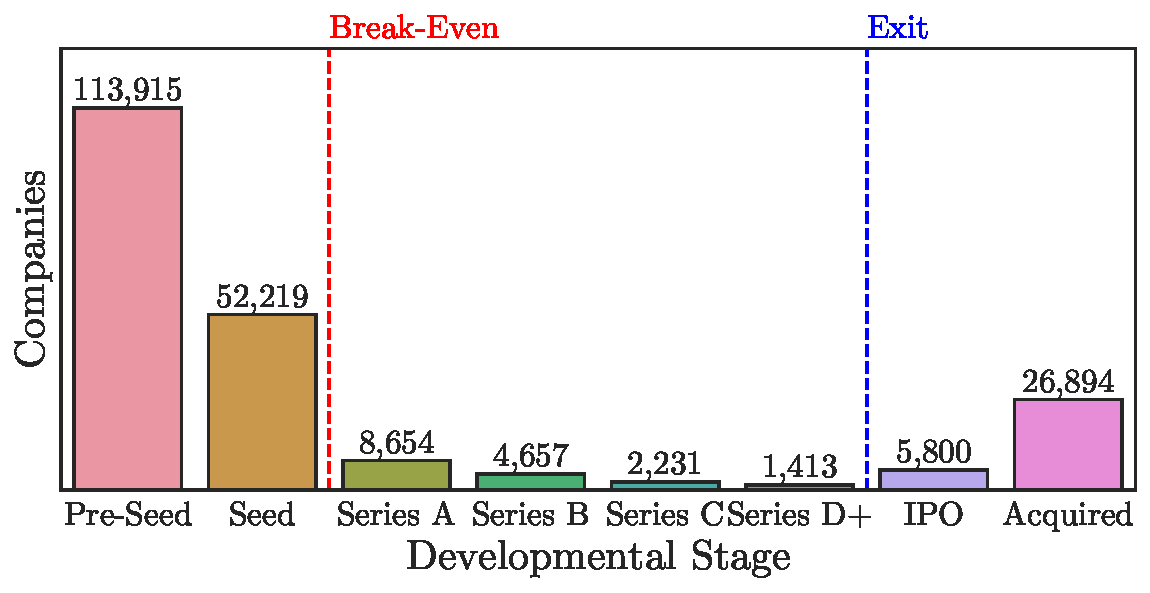
\includegraphics[width=\textwidth]{../figures/design/lifecycle}
    \caption[Startup development lifecyle]{Idealised startup development lifecycle (adapted, \cite{}) with company counts from the master dataset (c. September 2016). Red line represents profitability over time. The chart is divided into three periods: an early period of unprofitability (``Valley of Death'') where seed capital supports the business, a period of growth sustained by rounds of venture capital, and a transition to stability and mature capital markets.}
    \label{fig:design:lifecycle}
\end{figure}

After attempting to place the companies into development stages we are left with a large group of companies (the majority of the dataset) that have not raised funding and so can not be classified on that basis. We assume that companies that have not raised funding fall into two groups - those that intend to raise funding but have not had time to yet, and those that have chosen not to pursue funding and are unlikely to do so. We separated these groups by applying a cutoff equal to the 90th percentile of the age of companies in the Seed category, and excluded the older group from further analyses (N = 227,162,  53.3\%). As we are only interested in companies that could theoretically seek investment, we also excluded Closed, Acquired and IPO groups from further analyses (N = 35,973, 8.4\%).

Figure\ref{fig:design:stages_ages} depicts the ages of companies in the master dataset, grouped by developmental stage.  As we expected, there is a strong relationship between company stage and company age. Most pre-Series A companies are under five years old, and the majority of Series D+ funded companies are under 10 years old and the 75th percentile is at 15 years old. On this basis, we excluded companies that are over the 75th percentile of the age of companies in the Series D+ category (N =9,756, 2.2\%). Overall, our preliminary screening steps reduced the dataset from 425,934 companies to 153,043 companies, a reduction of 64.1\%.

\begin{figure}[!htb]
    \centering
    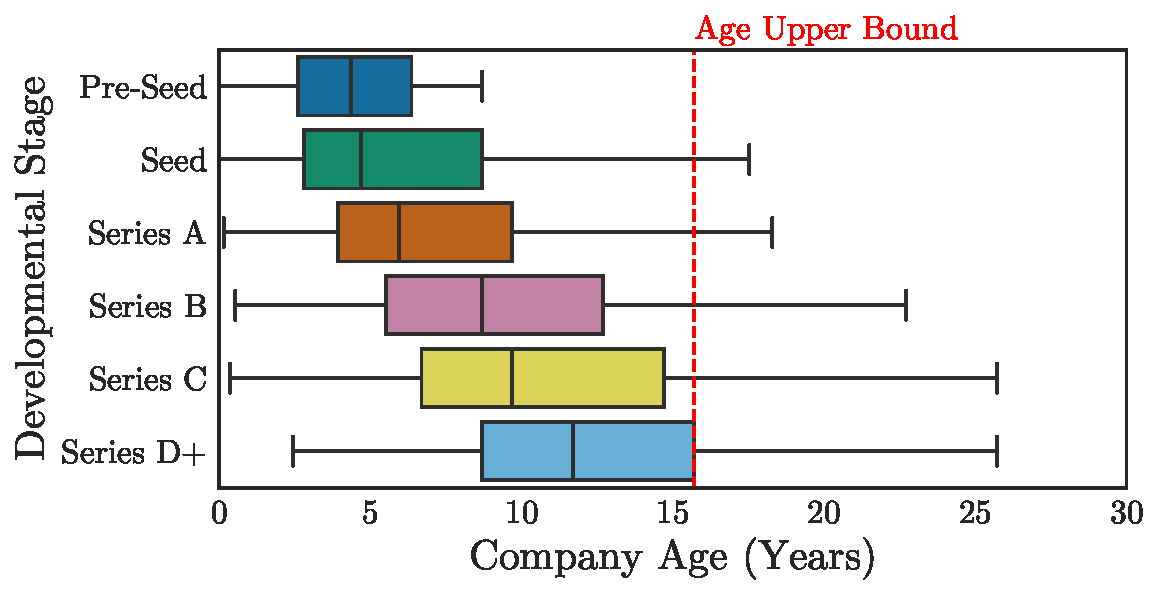
\includegraphics[width=\textwidth]{../figures/design/stages_ages}
    \caption[Company age distribution]{Company ages in years grouped by developmental stage. While there is significant variability in age for each developmental stage, there is a broad positive relationship between age and developmental stage. The dashed blue line represents the 75th percentile of the age of companies in the Series D+ category (15.7 years).}
    \label{fig:design:stages_ages}
\end{figure}

\subsection{Exploratory Analysis}

\subsubsection{Descriptive Statistics}

Table~\ref{fig:design:descriptive_statistics} presents the descriptive statistics for the dataset. The dataset is heavily skewed towards New companies (i.e. companies that were recently founded and have not raised any type of funding yet, 68.9\%). These companies have very few available features in comparison to companies at later developmental stages. We will investigate the impact of this sparsity on our predictions in Chapter~\ref{chap:evaluation}. We are presented with a fairly heterogenous dataset, the interquartile ranges imply significant variability in all measures. We do not believe that this implies that the data has not been cleaned effectively, but rather, reflects that startup companies naturally vary significantly in their traits.

\begin{table}[!htb]
    \centering
    \scalebox{0.9}{\begin{tabular}{lrrrrrrrrr} \toprule
& \multicolumn{1}{c}{Count} & \multicolumn{2}{c}{\thead{Age \\ (Years)}} & \multicolumn{2}{c}{\thead{Funding Raised \\ (USD, millions)}} & \multicolumn{2}{c}{\thead{Funding \\ Rounds (N)}} & \multicolumn{2}{c}{\thead{Available \\ Features (N)}} \\
Stage        & N         & Median & IQR   & Median & IQR   & Median & IQR   & Median & IQR   \\ \midrule
New          & 276,305   & 0.0    & 4.0   & 0.00   & 0.00  & 0.0    & 0.0   & 276    & 24    \\
Pre-Seed     & 8,850     & 3.0    & 3.0   & 0.05   & 0.41  & 1.0    & 0.0   & 319    & 30    \\
Seed         & 24,592    & 3.0    & 4.0   & 0.17   & 0.88  & 1.0    & 1.0   & 329    & 36    \\
Series A     & 7,966     & 4.0    & 5.0   & 4.00   & 7.71  & 2.0    & 1.0   & 341    & 40    \\
Series       & 4,028     & 6.0    & 6.0   & 14.00  & 20.71 & 2.0    & 2.0   & 349    & 43    \\
Series C     & 1,802     & 7.0    & 7.0   & 31.64  & 45.30 & 3.0    & 2.0   & 357    & 41    \\
Series D+/PE & 2,179     & 8.0    & 7.0   & 45.50  & 93.59 & 3.0    & 4.0   & 353    & 50    \\ \midrule
Total        & 325,722   & 1.0    & 5.0   & 0.0    & 0.0   & 0.0    & 0.0   & 278    & 37    \\
\bottomrule \end{tabular}
}
    \caption[Descriptive statistics]{Descriptive statistics grouped by developmental stage. Source: Master dataset (c. Sep-16).}
    \label{fig:design:descriptive_statistics}
\end{table}

CrunchBase's approach to industry classification is simplistic compared to other classification schemes (e.g., USSIC, NAICS, VentureSource) which generally have an industry hierarchy with tiers for broad industry sectors and sub-sectors providing further granularity. As a result, CrunchBase class labels include over represented and vague classes (e.g., ``Software'', ``Internet Services'') which could describe the majority of companies included in the database. In fact, ``Software'' and ``Internet Services'' account for 16.4\% and 13.4\% of all companies in the dataset respectively (see Figure~\ref{fig:design:industry_counts}). Despite these vague class labels, it is clear the dataset skews towards high technology startups, as opposed to biomedical, agricultural, or other technologies.

\begin{figure}[!htb]
    \centering
    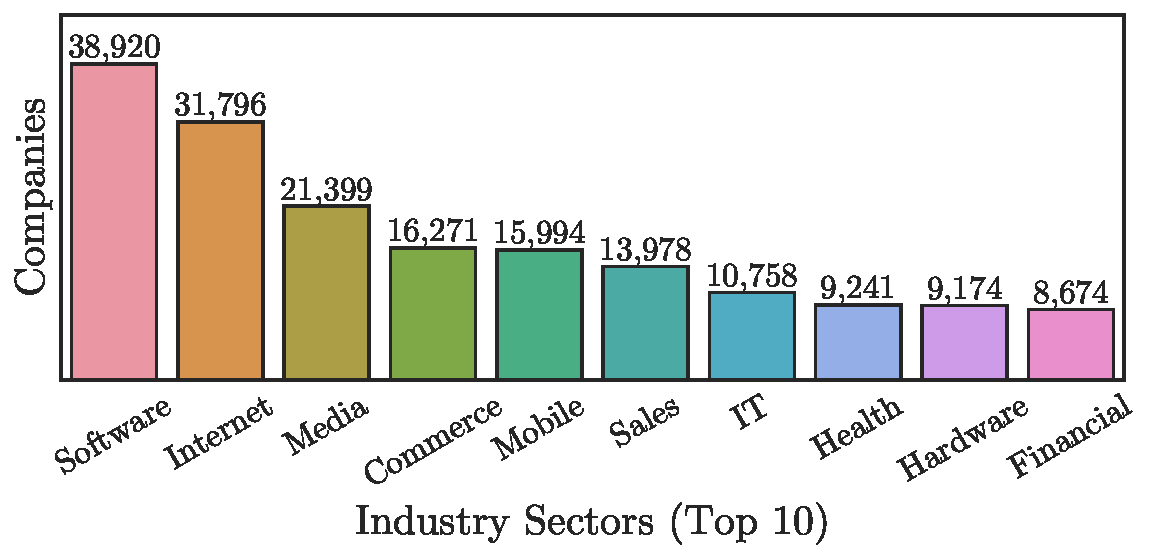
\includegraphics[width=\textwidth]{../figures/design/industry_counts}
    \caption[Companies by industry sector]{Companies grouped by industry sector. The 10 most common sectors are displayed. Source: Master dataset (c. September 2016).}
    \label{fig:design:industry_counts}
\end{figure}

\subsubsection{Sparsity}

First, we explored missing data in the dataset. We expected the dataset to be highly sparse because it primarily came from CrunchBase, a crowd-sourced database. As profiles are entered into CrunchBase piece-meal, it is not clear at face-value whether data (e.g. records of funding rounds) is missing or didn't occur. Figure~\ref{fig:design:sparsity} displays the distribution of missing data in the dataset, with respect to each feature and each feature. The multi-modal peaks of both distributions suggest that missing data across certain groups of features may be correlated with each other (e.g. all features derived from funding rounds).

\begin{figure}[!htb]
    \centering
    \begin{subfigure}{\textwidth}
        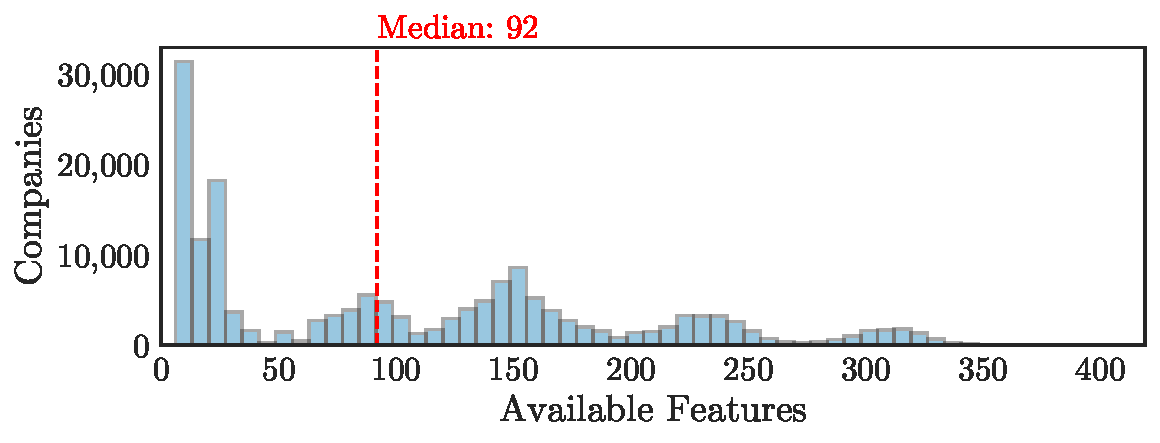
\includegraphics[width=\textwidth]{../figures/design/sparsity_features}
        \caption[Sparsity by company]{Distribution of missing data by company}
        \label{fig:design:sparsity:features}
    \end{subfigure}
    \begin{subfigure}{\textwidth}
        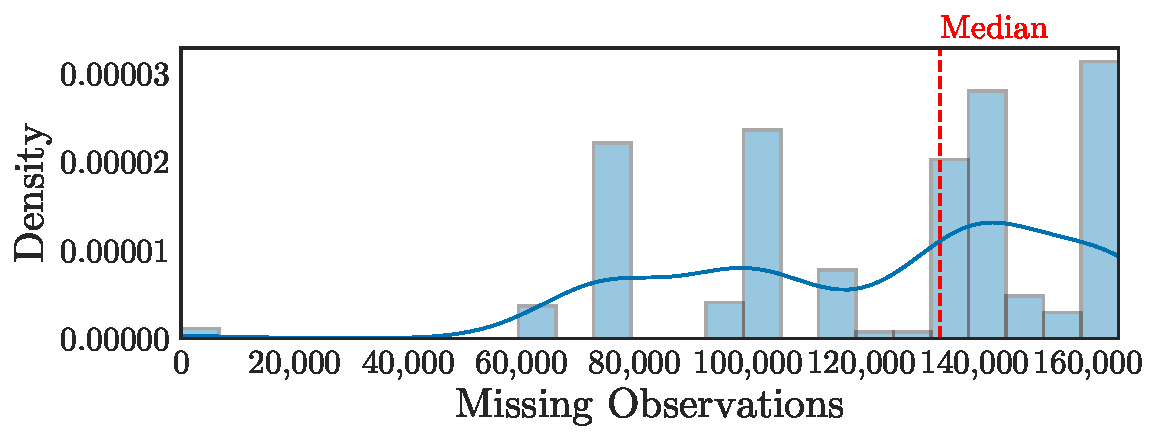
\includegraphics[width=\textwidth]{../figures/design/sparsity_observations}
        \caption[Sparsity by feature]{Distribution of missing data by feature}
        \label{fig:design:sparsity:observations}
    \end{subfigure}
    \caption[Dataset sparsity]{Distribution of missing data in master dataset (c. September 2016).}
    \label{fig:design:sparsity}
\end{figure}

\subsubsection{Normality}

Next, we explored the distributions of features. Figure~\ref{fig:design:normality} shows the skewness and kurtosis of the features in our dataset. A feature is considered horizontally symmetrical if it has a skewness of 0 and generally considered highly skewed if its absolute skewness is above 1 \cite{bulmer1979}. The vast majority of our features are more skewed than this cutoff. Kurtosis is a measure of the distribution of variance in a feature. We use Fisher's measure of kurtosis, which has a normal value of 0. Our dataset has consistently higher kurtosis than normal which suggests that we have many extreme values in our dataset. These results in concert suggest that our dataset has many features that are positively skewed with long-tail distributions. This is intuitively what we might expect for features like ``amount of funding raised''.

\begin{figure}[!htb]
    \centering
    \begin{subfigure}{\textwidth}
        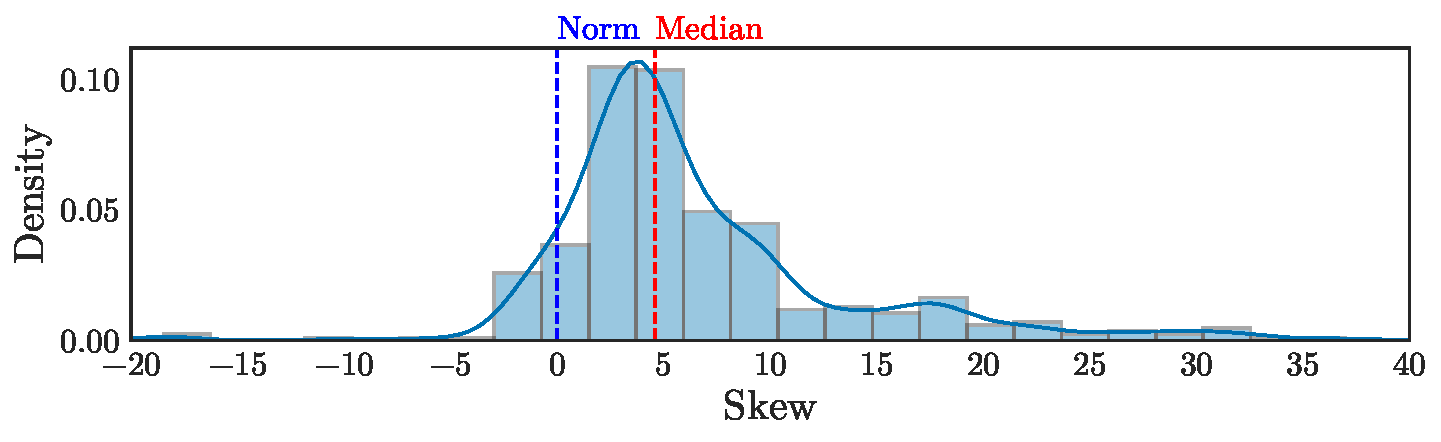
\includegraphics[width=\textwidth]{../figures/design/skew}
        \caption{Distribution of skew by feature}
        \label{fig:design:normality:skew}
    \end{subfigure}
    \begin{subfigure}{\textwidth}
        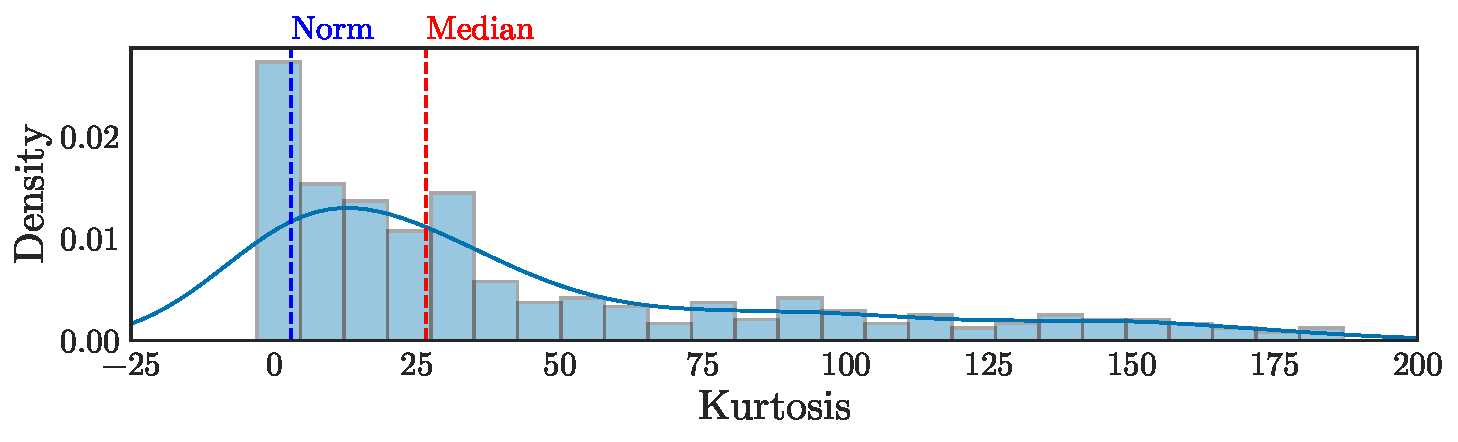
\includegraphics[width=\textwidth]{../figures/design/kurtosis}
        \caption{Distribution of kurtosis by feature}
        \label{fig:design:normality:kurtosis}
    \end{subfigure}
    \caption[Dataset normality]{Distribution of features in master dataset (c. September 2016).}
    \label{fig:design:normality}
\end{figure}

\subsubsection{Scale}

Next, we explored the scaling and range of each of our features. Figure~\ref{fig:design:scaling} shows the \gls{iqr} of each feature (transformed by log1p for ease of viewing). The distribution is extremely skewed, which shows that our features have very different scaling. This may be an issue for our machine learning estimators and feature extractors, so we address this by applying a scaler in our pipeline.

\begin{figure}[!htb]
    \centering
    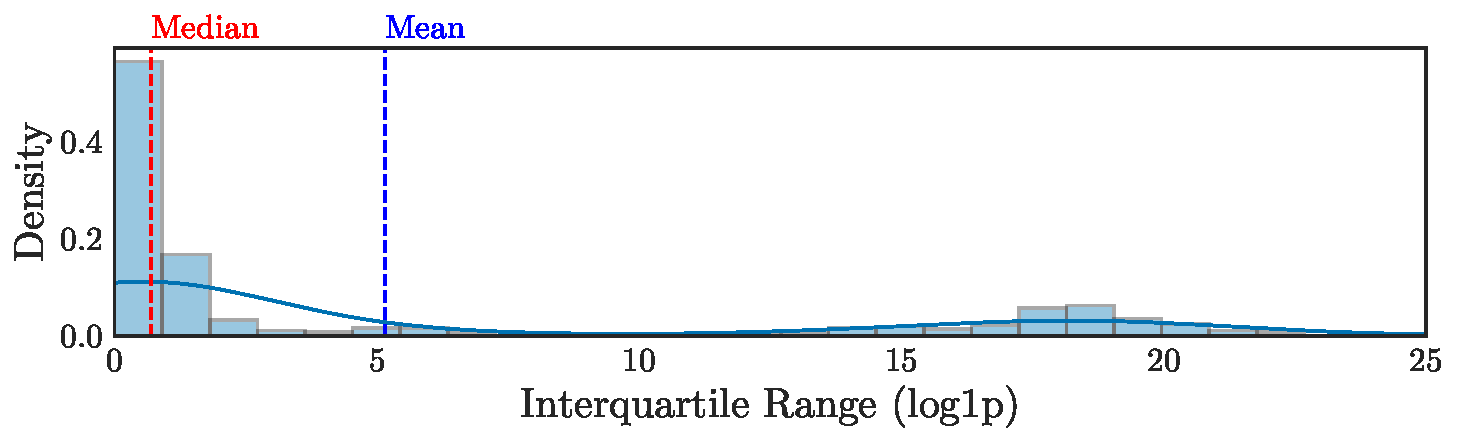
\includegraphics[width=\textwidth]{../figures/design/scaling}
    \caption[Dataset feature scaling]{Distribution of interquartile ranges (transformed by log1p) in master dataset (c. September 2016).}
    \label{fig:design:scaling}
\end{figure}

\subsubsection{Orthogonality}

Finally, we explored the orthogonality of our features: the extent to which the variance of our features is unrelated. This is a less straight-forward measure. We explore pair-wise inter-correlations between our features and evaluate how many of the inter-correlations are above a particular correlation cutoff, as depicted in Figure~\ref{fig:design:orthogonality}. We use two correlation metrics: Pearson and Spearman. Pearson is more commonly used but Spearman is a ranked metric and may more accurately reflect our non-normal feature distributions. Although most features have relatively low inter-correlations (\~60\% below 0.2) there are still a considerable number that are highly correlated, so it might be efficient to remove these features using an unsupervised feature extracter prior to estimation.

\begin{figure}[!htb]
    \centering
    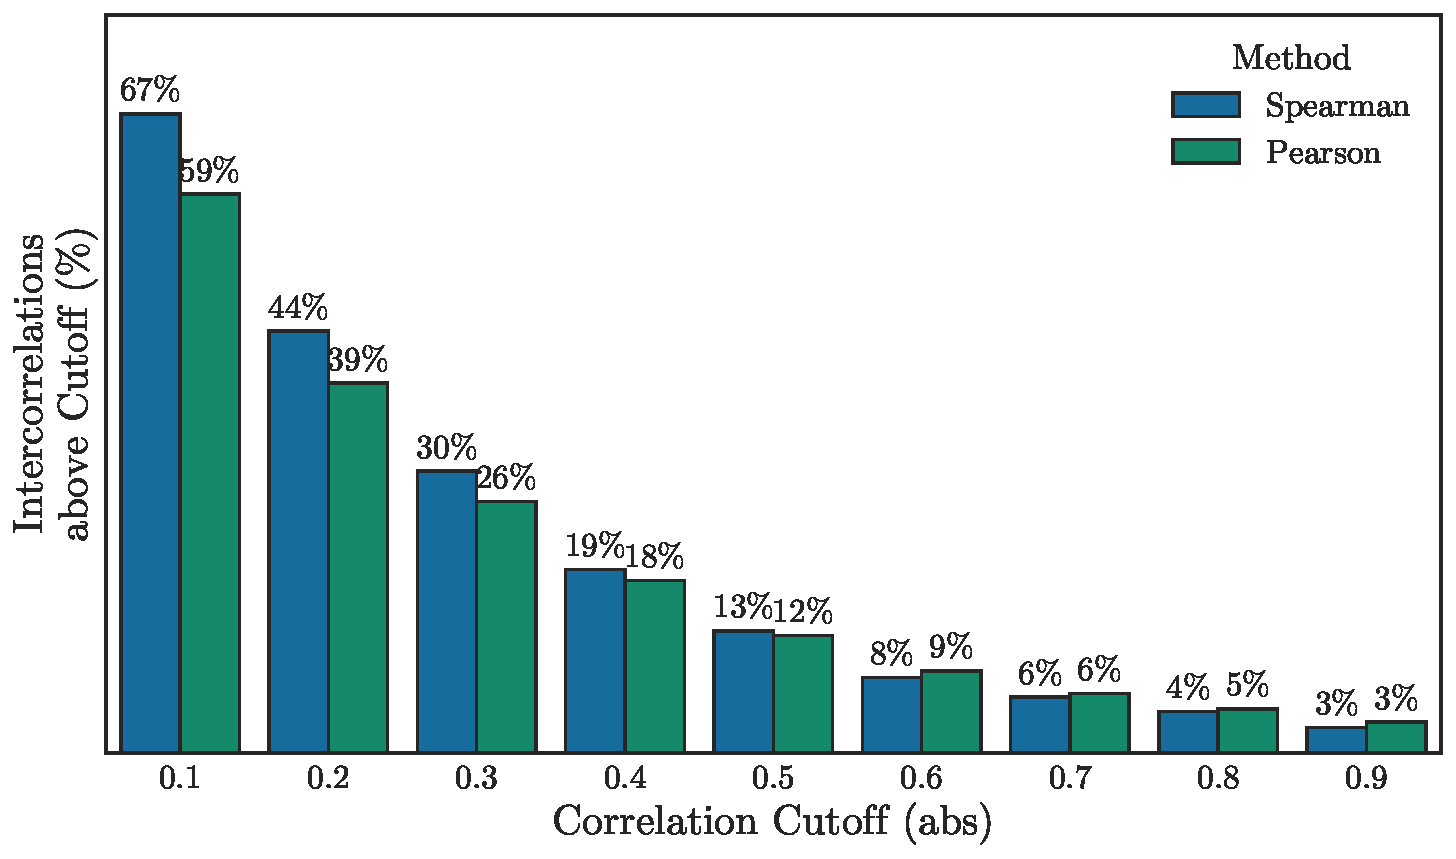
\includegraphics[width=\textwidth]{../figures/design/orthogonality}
    \caption[Dataset orthogonality]{Distribution of intercorrelations in master dataset (c. September 2016).}
    \label{fig:design:orthogonality}
\end{figure}

\section{Pipeline Creation}

We developed a classification pipeline using the popular Python-based machine learning library Scikit-learn \cite{pedregosa2011}. The classification pipeline construct allows us to easily search across hyperparameters at each step in the pipeline (see Appendix~\ref{appendix:pipeline_hyperparameters} for hyperparameter list). The following sections explore the testing of each hyperparameter decision, and the selection of primary classifiers for the following steps. This process is depicted in Figure~\ref{fig:design:pipeline_creation}.

\begin{figure}[!htb]
    \centering
    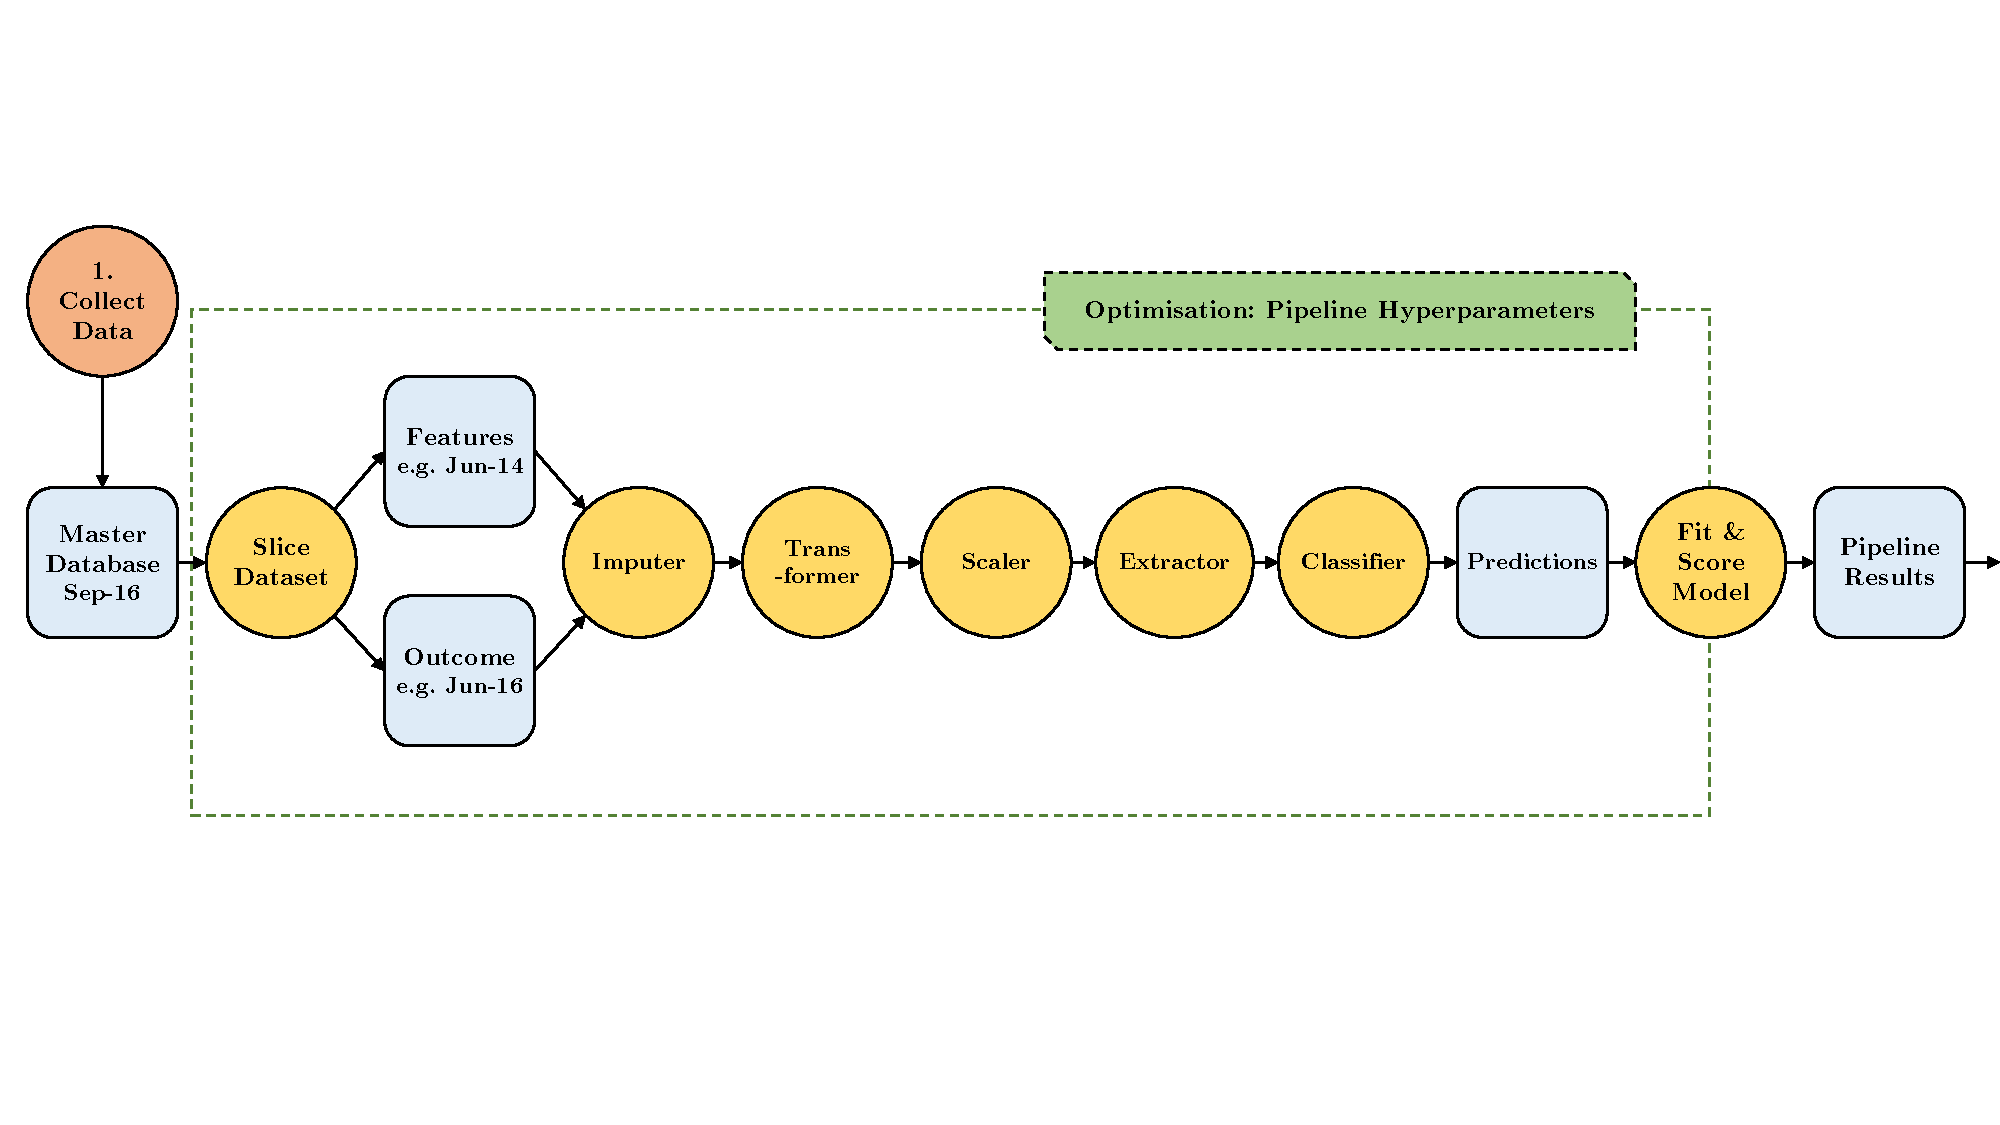
\includegraphics[width=\textwidth]{../figures/design/pipeline_creation}
    \caption[Pipeline creation flowchart]{Pipeline creation overview.}
    \label{fig:design:pipeline_creation}
\end{figure}

\subsection{Imputation}

After reviewing the distribution of missing data, we decided to perform further investigation into imputation methods. Common imputation strategies include replacing missing values with the mean, median or mode of each feature. Figure~\ref{fig:design:central_tendency} shows the distribution of mean, median and modes for each feature in the dataset. For the majority of features, all three measures of central tendency are equal to zero. This resolves the issue of distinguishing missing data from negative observations because, following imputation, all of these data points will map to zero. Figure~\ref{fig:design:imputer} shows the receiver-operating characteristics of the different imputation strategies. As expected, all three imputation strategies produce similar results (within the margin of error).

\begin{figure}[!htb]
    \centering
    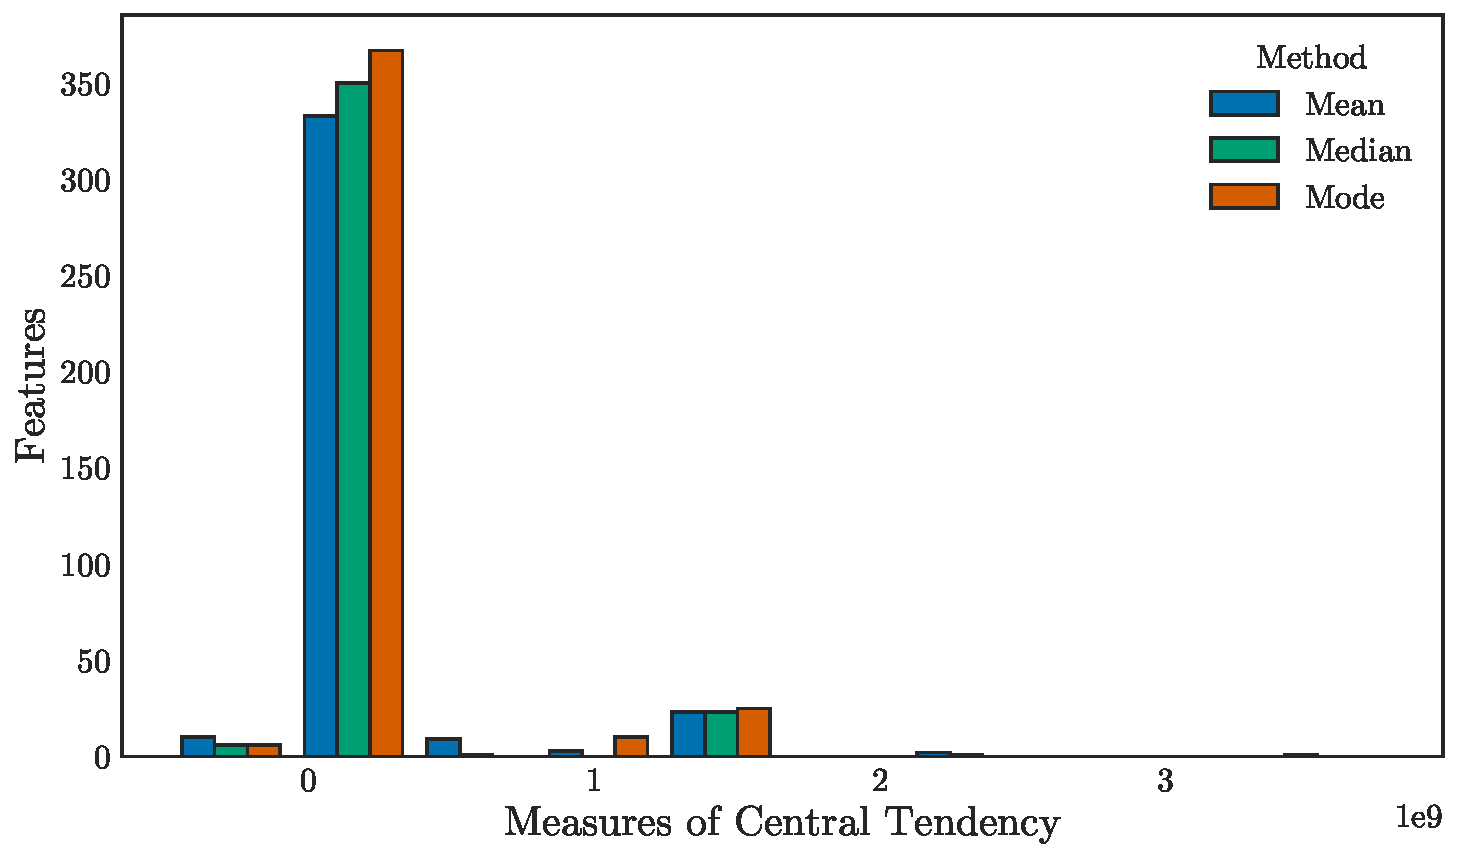
\includegraphics[width=\textwidth]{../figures/design/central_tendency}
    \caption[Imputation replacement values]{Distribution of measures of central tendency (mean, median and mode) in master dataset (c. September 2016).}
    \label{fig:design:central_tendency}
\end{figure}

\begin{figure}[!htb]
    \centering
    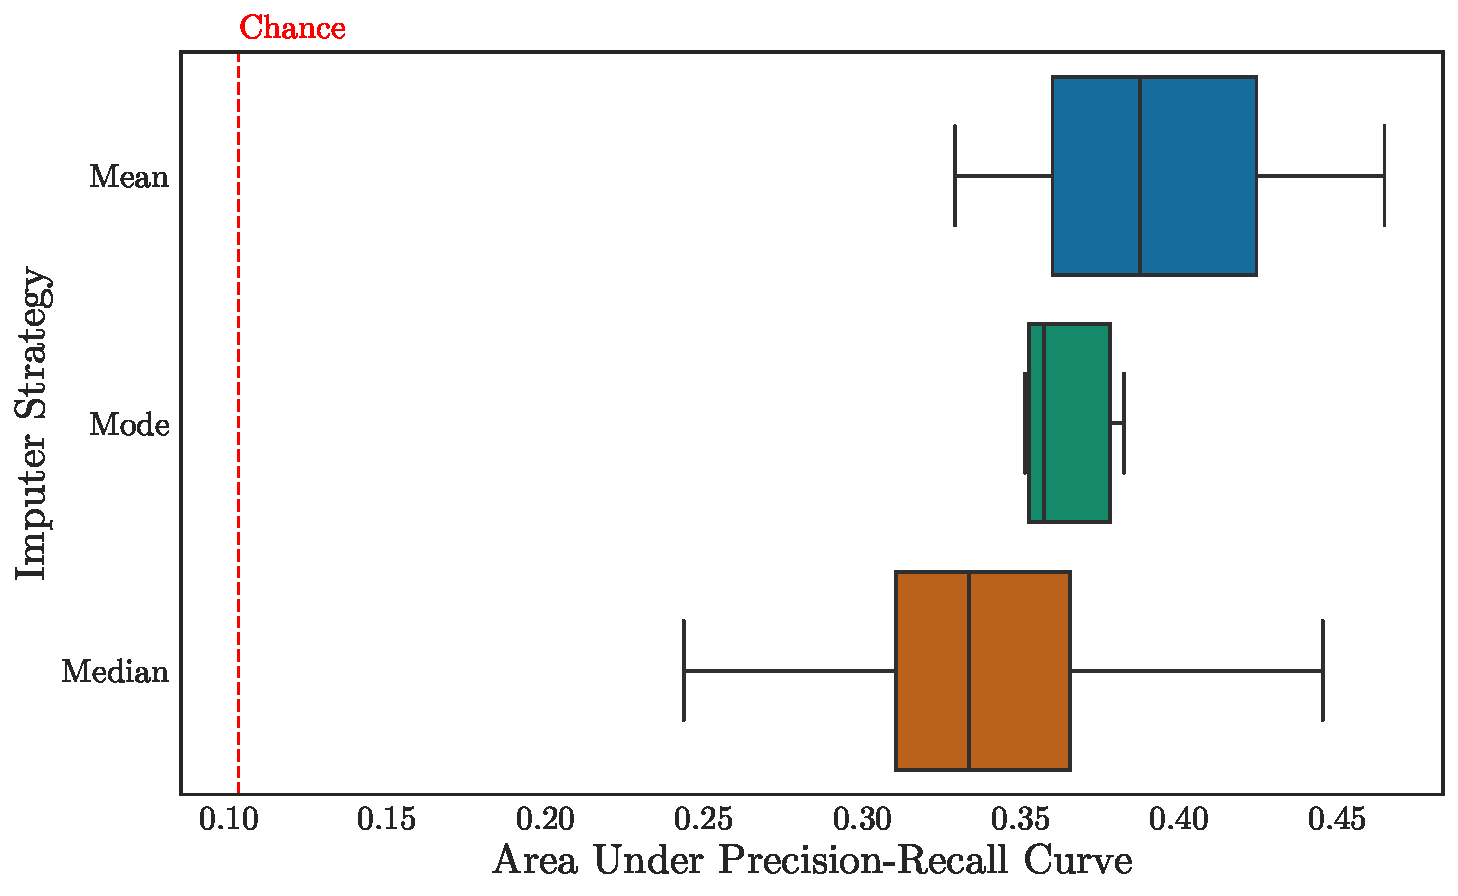
\includegraphics[width=\textwidth]{../figures/design/imputer}
    \caption[Area under PR Curves by imputation strategy]{Area under \gls{roc} for different imputation strategies. Imputation strategies include replacing missing values with the most frequent (mode), median and mean value of each respective feature. Results presented are aggregated from hyperparameter optimisation performed over entire classification pipeline (including all classifiers).Source: Features (Apr-12) and labels (Apr-14, 2 year forecast window) derived from Master dataset (c. Sep-16).}
    \label{fig:design:imputer}
\end{figure}

\subsection{Transformation}

While the classification algorithms we identified in the previous chapter are relatively robust to violations of normality, it may be beneficial to transform the data if the feature distributions are extreme. Table~\ref{fig:design:funding_transformation} shows one of the key features, Total Funding Raised, under a number of different transformations. Like many features in our dataset, the distribution of Total Funding Raised is highly skewed. The log transformation reduces this skew (a normal distribution of non-zero values is apparent) and square root transformation also reduces this skew (to a lesser extent). The impact of these transformations is reduced by the extent of their zero-inflation. However, it is still reasonable to expect both of these transformations to improve the classification accuracy. Figure~\ref{fig:design:transformer} shows the \gls{roc} of these different transformation functions. Both functions provide a small performance improvement, with the square root function narrowly best.

\begin{table}[!htb]
    \centering
    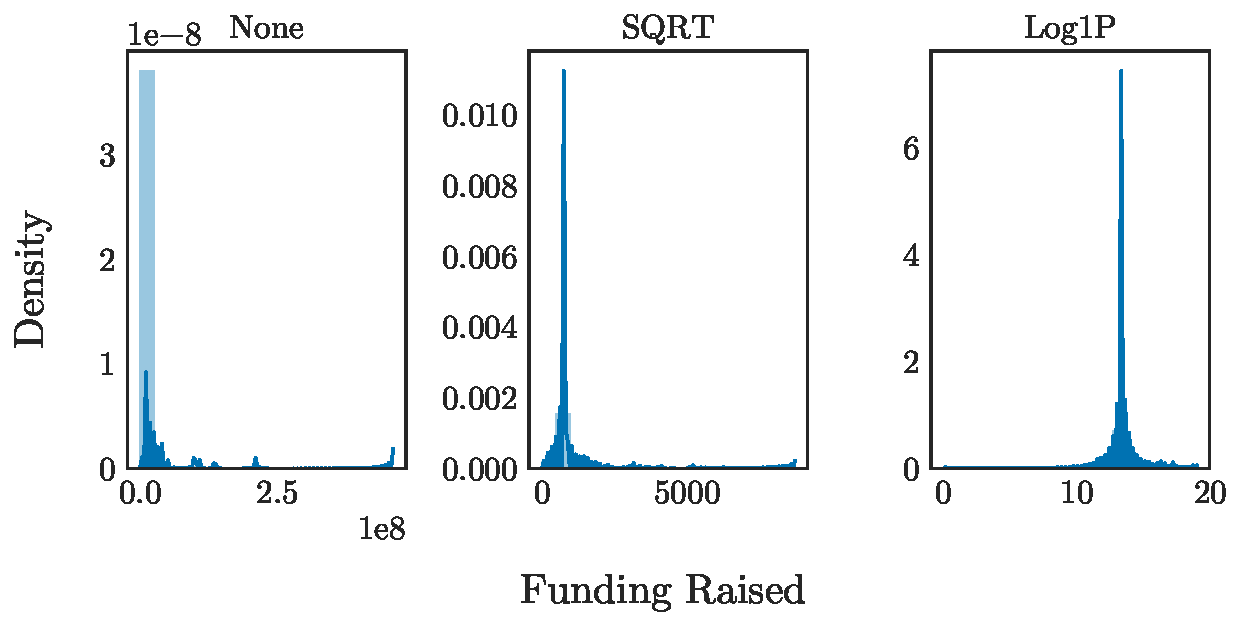
\includegraphics[width=\textwidth]{../figures/design/funding_transformation}
    \caption[Example feature under transformation functions]{}
    \label{fig:design:funding_transformation}
\end{table}

\begin{figure}[!htb]
    \centering
    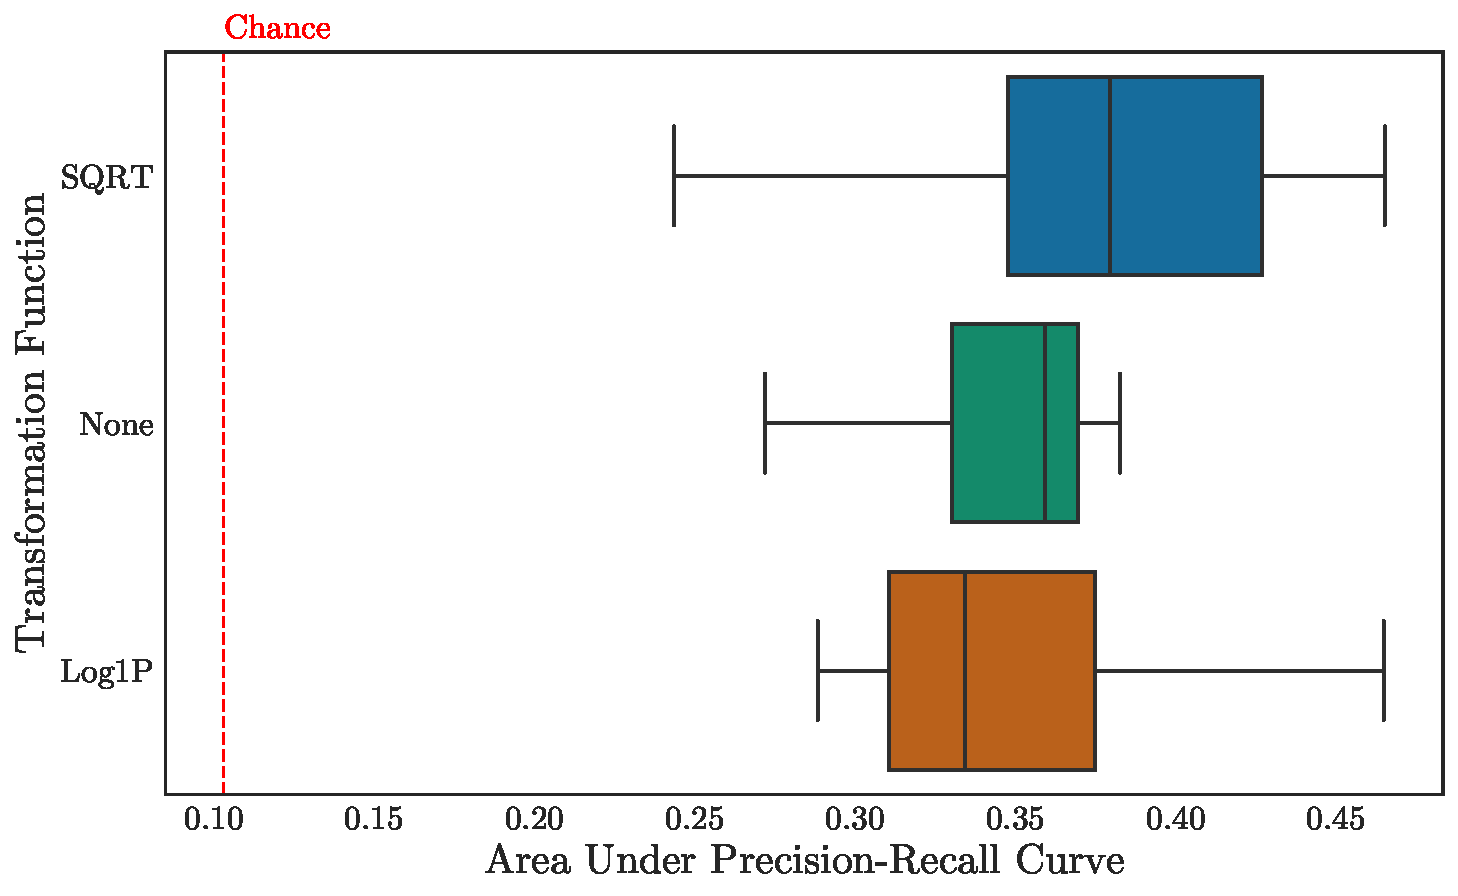
\includegraphics[width=\textwidth]{../figures/design/transformer}
    \caption[Area under PR Curves by transformation function]{Area under \gls{roc} for different transformation functions. Transformations include: None (identity transformation), Log1p (natural logarithm of one plus the input array, element-wise), and Sqrt (the square root of the input array, element-wise). Results presented are aggregated from hyperparameter optimisation performed over entire classification pipeline (including all classifiers).Source: Features (Apr-12) and labels (Apr-14, 2 year forecast window) derived from Master dataset (c. Sep-16).}
    \label{fig:design:transformer}
\end{figure}

\subsection{Scaling}

Standardisation of datasets is a common requirement for many feature extraction methods and machine learning estimators. Sci-kit learn provides three primary scaling functions: StandardScaler, RobustScaler and MinMaxScaler. RobustScaler is intended to alleviate the effect of outliers while MinMaxScaler is intended to preserve zero entries in sparse data - both of these are relevant properties for the dataset. Figure~\ref{fig:design:scaler} shows the receiver-operating characteristics of the different scaling functions. MinMaxScaler and RobustScaler actually underperform the null condition while StandardScaler only performs on par with the null condition. This is unexpected but may be caused by the previously applied transformations.

\begin{figure}[!htb]
    \centering
    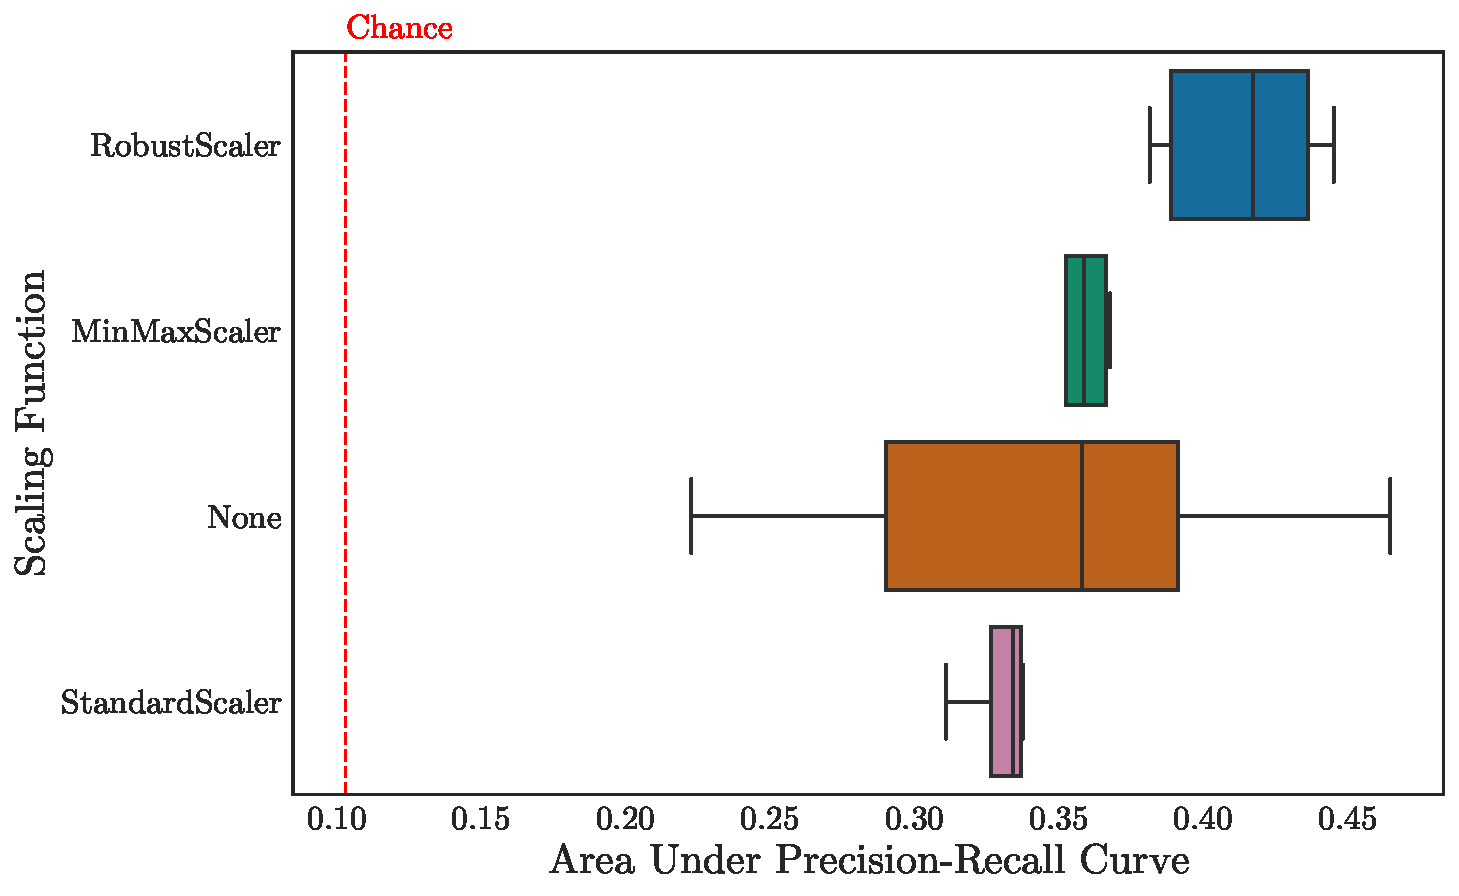
\includegraphics[width=\textwidth]{../figures/design/scaler}
    \caption[Area under PR Curves by scaling function]{Area under \gls{roc} for different scaling functions. Scaling functions include: None, StandardScaler (mean: 0, variance: 1), RobustScaler (median: 0, IQR: 1) and MinMaxScaler (min: 0, max: 1). Results presented are aggregated from hyperparameter optimisation performed over entire classification pipeline (including all classifiers).Source: Features (Apr-12) and labels (Apr-14, 2 year forecast window) derived from Master dataset (c. Sep-16).}
    \label{fig:design:scaler}
\end{figure}

\subsection{Extraction}

Feature extraction reduces high-dimensional data into lower-dimensional data in such a way that maximises the variance of the data. The most common approach to dimensionality reduction is \gls{pca}, which constructs orthogonal eigenvectors (components). The magnitude of each eigenvector (its eigenvalue) is displayed in Figure~\ref{fig:design:scree_plot}. The majority of explained variance is captured in the first 10 components, and the Eigenvalues drop below 1 by 100 components - this suggests that these are reasonable values for further hyperparameter search. Figure~\ref{fig:design:extracter} shows the \gls{roc} for different numbers of extracted components. All curves produce similar classification results (within margin of error) which implies that we should extract between 1 -- 20 components because it will provide us with more efficient computation.

\begin{figure}[!htb]
    \centering
    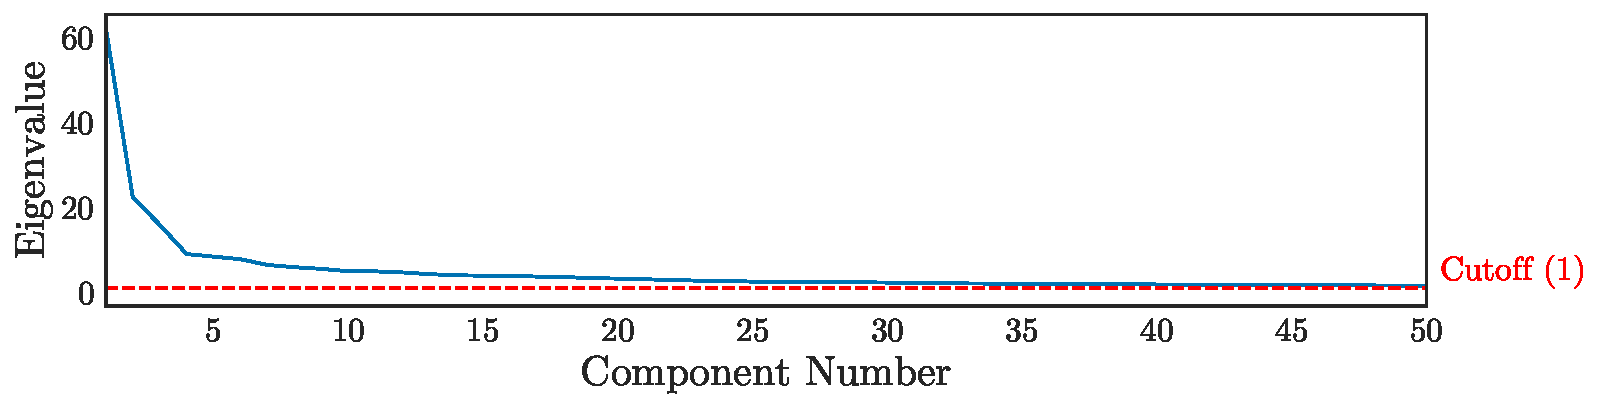
\includegraphics[width=\textwidth]{../figures/design/scree_plot}
    \caption[PCA Scree Plot]{Eigenvalues extracted from \gls{pca} model. Horizontal line drawn at an Eigenvalue of 1 -- this theoretically represents the ‘contribution’ of one original feature and is commonly used as an approximate threshold for included components. Source: Master dataset (c. Sep-2016).}
    \label{fig:design:scree_plot}
\end{figure}

\begin{figure}[!htb]
    \centering
    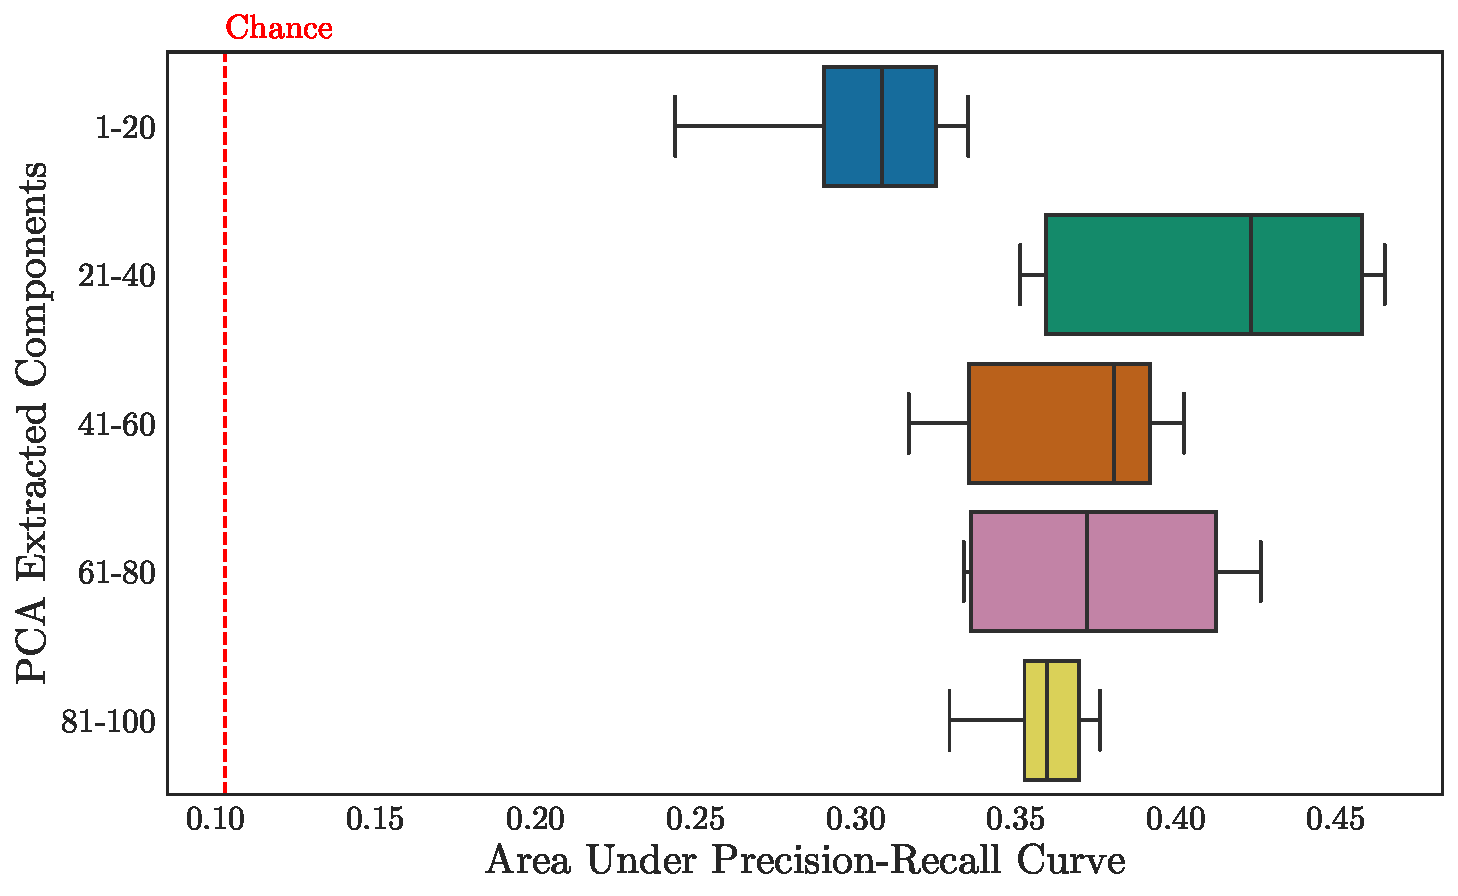
\includegraphics[width=\textwidth]{../figures/design/extracter}
    \caption[Area under PR Curves by PCA techniques]{Area under \gls{roc} for different number of extracted components from \gls{pca}. Curves have been grouped by the quotient of the number of components divided by 20 to result in five ordered groups (e.g. Range [0, 19] --> 0). Results presented are aggregated from hyperparameter optimisation performed over entire classification pipeline (including all classifiers).Source: Features (Apr-12) and labels (Apr-14, 2 year forecast window) derived from Master dataset (c. Sep-16).}
    \label{fig:design:extracter}
\end{figure}

While \gls{pca} is efficient at reducing features, the resultant components are not interpretable. Similarly, individual analysis of 400+ features is difficult to interpret. A compromise is to group the features using the conceptual framework we developed earlier from the literature review. The grouping approach applied weights to each individual feature that optimised the inter-correlations within each group. Given the highly skewed features, we use Spearman correlation which is robust to skewness because it is based on ranking. Figure~\ref{fig:design:grouped_heatmap} displays the inter-correlations between each factor from the proposed conceptual framework. As we would expect, `investors' and `funding' features are highly correlated. While `investors' attempts to capture the influence of previous investors, it also captures features like the size of an investor's past investments, which would likely correlate with the size of the investment they made in the target company. Interestingly, `founders' features are positively correlated with all other features except for `advisors' features which are negatively correlated with all other feature groups.

\begin{figure}[!htb]
    \centering
    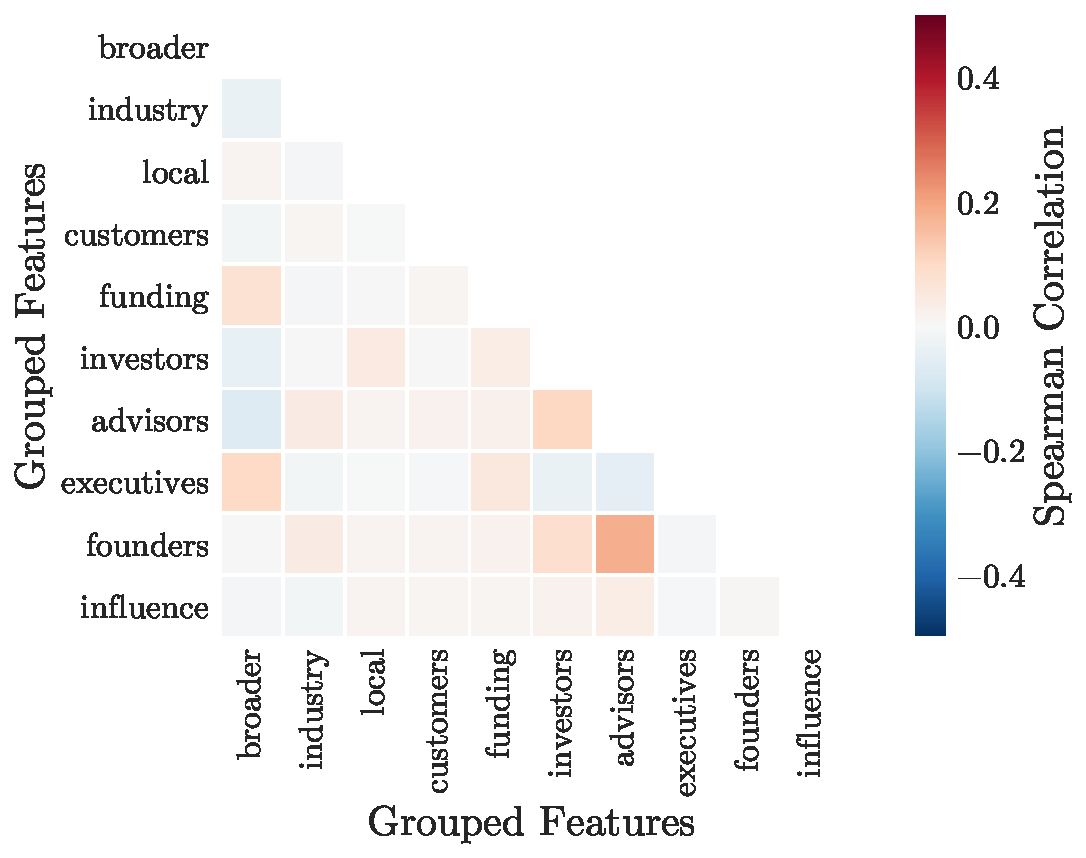
\includegraphics[width=\textwidth]{../figures/design/grouped_heatmap}
    \caption[Inter-correlations of factors from framework]{Inter-correlations of each factor from conceptual framework. Spearman ranking correlation is used. Individual features are grouped by applying weights that maximise the inter-correlations within each group from our conceptual framework (see Figure 2.1). Source: Master dataset (c. Sep-2016).}
    \label{fig:design:grouped_heatmap}
\end{figure}

\subsection{Classification Algorithms}

The literature review we performed in the previous chapter revealed seven common supervised classification algorithms potentially suitable for application to this problem area. Our review suggested that Random Forests were most likely to provide a successful trade-off between predictive power, interpretability and time taken. We empirically tested each of these classifiers and compared their performance against a range of metrics, as displayed in Table~\ref{fig:design:classification_metrics}. We report maximum as well as median recorded scores to ensure we didn't penalise algorithms that had unfavourable hyperparameter search spaces.

\begin{table}[!htb]
    \centering
    \scalebox{0.8}{\begin{tabular}{lrrrrr} \toprule
                            & ROC        & PRC        & F1         & MCC        & Time (s) \\
Classifier                  & Max        & Max        & Max        & Max        & Median \midrule
Random Forest               & \em{0.780} & \em{0.471} & \em{0.324} & \em{0.300} & 55.1
Logistic Regression         & 0.766      & 0.445      & 0.286      & 0.293      & 14.9
Decision Tree               & 0.753      & 0.456      & 0.265      & 0.249      & 15.9
Naive Bayes                 & 0.713      & 0.383      & 0.297      & 0.259      & 26.5
Support Vector Machine      & 0.605      & 0.525      & 0.266      & 0.300      & 746.2
Artificial Neural Network   & 0.609      & 0.313      & 0.241      & 0.243      & 15.9
K-Nearest Neighbors         & 0.545      & 0.340      & 0.157      & 0.203      & \em{10.0}
\bottomrule \end{tabular}
}
    \caption[Overview of classification algorithm performance]{}
    \label{fig:design:classification_metrics}
\end{table}

We take a closer look at the \gls{pr} curves for each classifier in Figure~\ref{fig:design:classifier}. While all classifiers perform better than chance, Logistic Regressions and Random Forests come out ahead, and Support Vector Machines and Artificial Neural Networks appear to underperform. Delving into the cross-validated learning curves for each classifier (Figure~\ref{fig:design:create_learning_curves}) we see that Naive Bayes, Logistic Regression, Artificial Neural Networks and Support Vector Machines quickly converge, whereas Decision Trees, Random Forests and K-Nearest Neighbors require more observations to converge. This suggests that we might expect Random Forests to do better in final testing (as testing will not be cross-validated), as well as in the future as the dataset naturally grows.

\begin{figure}[!htb]
    \centering
    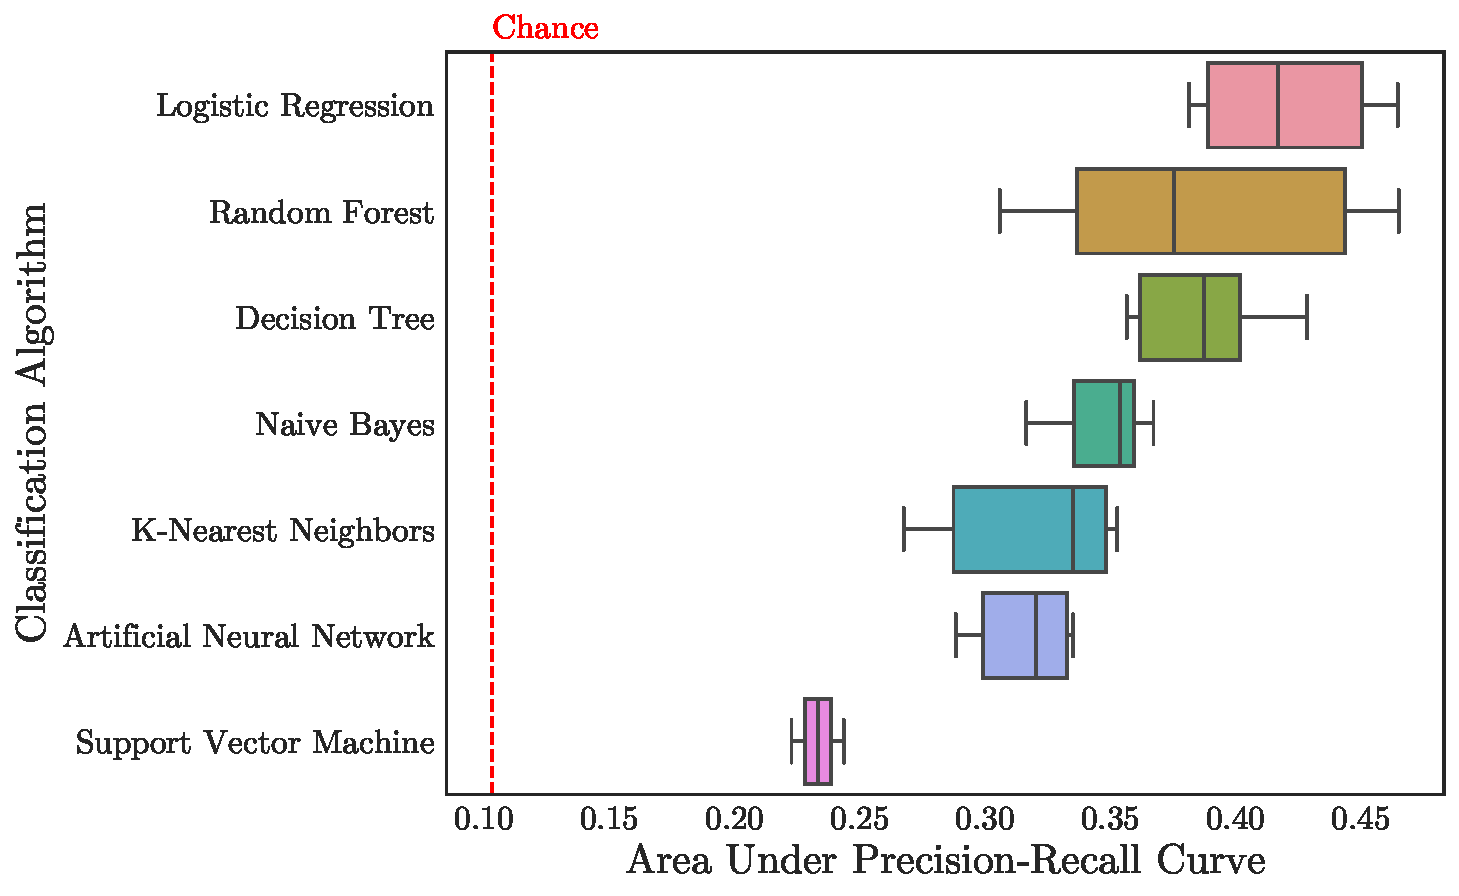
\includegraphics[width=\textwidth]{../figures/design/classifier}
    \caption[Area under PR Curves by classification algorithms]{Area under \gls{roc} for different classification algorithms. All algorithms are implementations from the Sci-kit learn library. Results presented are aggregated from hyperparameter optimisation performed over entire classification pipeline (including all classifiers).Source: Features (Apr-12) and labels (Apr-14, 2 year forecast window) derived from Master dataset (c. Sep-16).}
    \label{fig:design:classifier}
\end{figure}

\begin{figure}[!htb]
    \centering
    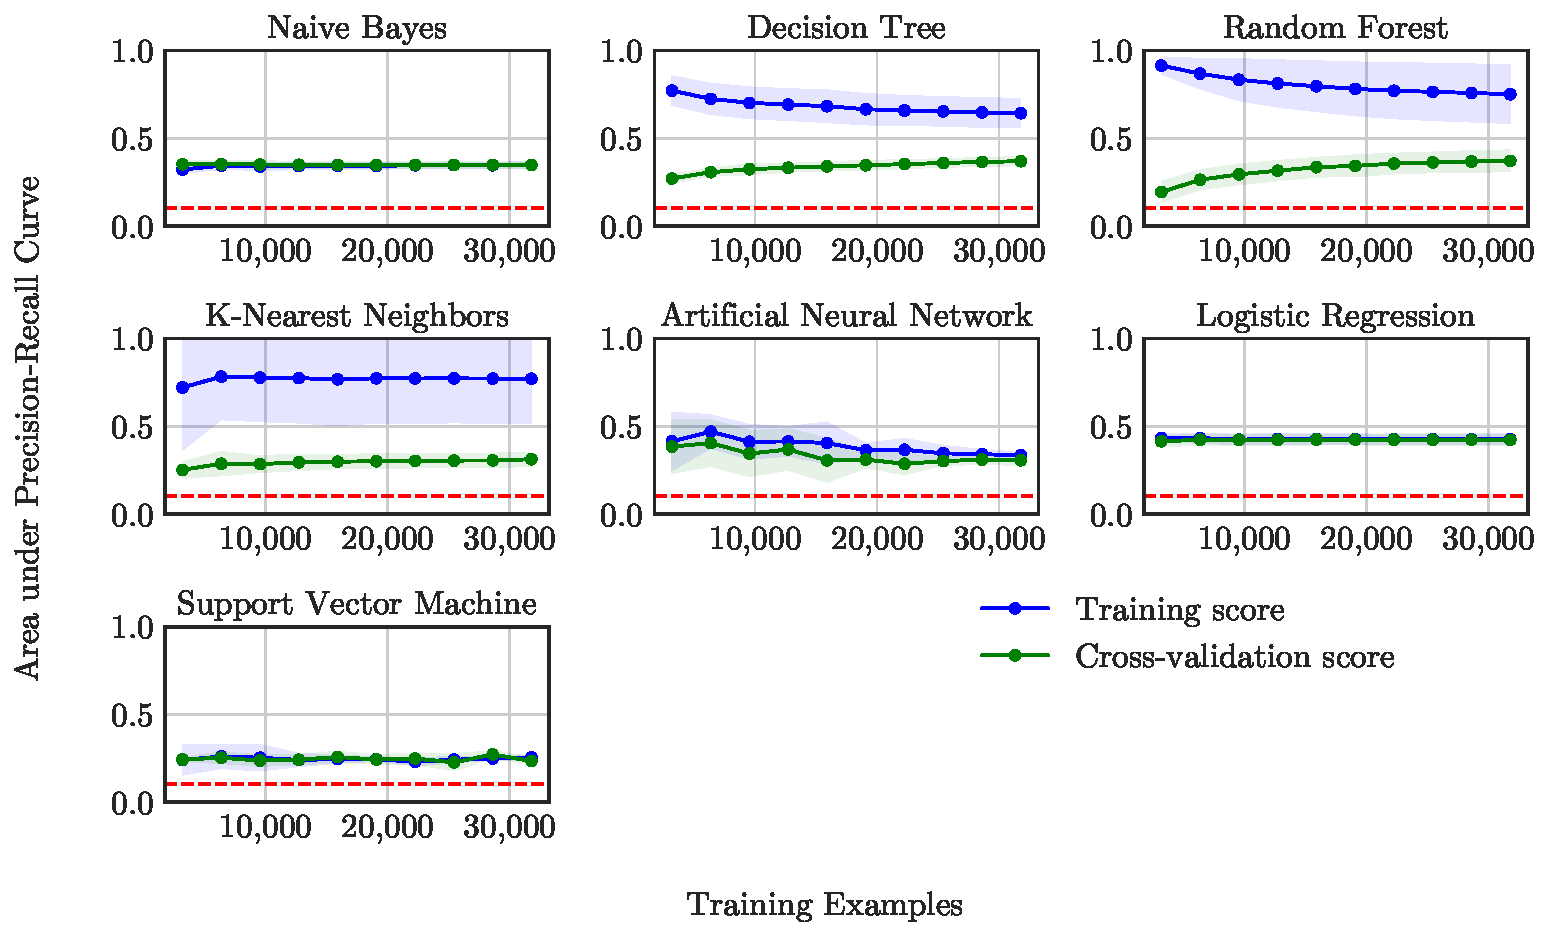
\includegraphics[width=\textwidth]{../figures/design/create_learning_curves}
    \caption[Learning curves by classification algorithms]{Learning curves.}
    \label{fig:design:create_learning_curves}
\end{figure}

\ifcsdef{mainfile}{}{\printbibliography}
\end{document}
